Following the integration of updated high temperature opacities detailed in \S
\ref{sec:p1}, we will investigate using the observed color and magnitude range
of the Jao Gap to age-date kinematically seperated populations within the solar
neighboorhood.

While low-mass stars provide the majority of the fitting points for isochrones
when estimating ages of clusters, due to the very slow variations in
observables during main sequence evolution, it remains challenging to measure
precise and accurate ages for low mass field stars \citep{Soderblom2010,
Veyette2018, Kiman2021}. Moreover, the extremely high density of isochrones
near the ZAMS, can result in uncertainties on isochrone age estimates for K
and M dwarfs as high as 50 \% \citep{Lu2021}. As a result of these high
isochrone age uncertainties other methods of dating non-cluster populations
have been developed, including age-calibrated rotation-activity relations
\citep[e.g.][]{Kiman2021} and gyro-kinematic age-dating \citep[e.g.][]{Lu2021}.
In this chapter of the thesis we will present both a method of calibrating a
Jao Gap location -- age relation alongside a study of the mechanism driving a
population's Jao Gap location to evolve with age.

Both preliminary modeling and literature
\citep[e.g.][]{Jao2018,Jao2020,Feiden2021,Mansfield2021} demonstrate that the
Jao Gap is expected to migrate along the main sequence as a population of stars
age. Our modeling indicates that stellar populations younger than $\sim 2$ Gyr
do not show a gap. However, once the gap forms it will migrate towards bluer
portions of the CMD with age.

For this proposal we do not perform any rigorous statistical testing of whether
the differences in theoretical Jao Gap location could be discrimated between in
observational data; instead, choosing to save that element of the research for
thesis work proper. However, we do perform a qualitative test of the visual
distinguisability of the Jao Gap location in two CMDs with different sample
sizes --- 500 and 1000 stars (Figure \ref{fig:JGTTE}).

We evolve models over an extremely finely sampled mass grid centered at the
theoretical Jao Gap location for a GS98 solar composition population of stars.
We then adopt the \citep{Sollima2019} IMF between 0.1 and 1 $M_{\odot}$
(Equation \ref{eqn:IMF}) to sample these evolved models. Model surface
gravities, effective temperatures, and luminosities are transformed into Gaia
magnitudes using bolometric correction tables provided by
ESA\footnote{\url{https://gea.esac.esa.int/archive/documentation/GDR2/Data\_processing/chap\_cu5pho/sec\_cu5pho\_calibr/ssec\_cu5pho\_calibr\_extern.html}}
and color-code provided by Dotter. 

\begin{equation}\label{eqn:IMF}
	\xi(m) = \xi_{0}\left(\frac{m}{M_{\odot}}\right)^{-2.68\pm0.09}
\end{equation}

% Uncertainty is injected by first
% transforming $G$, $BP$, and $RP$ flux and flux uncertaninty measurments for all
% sources Gaia DR3 reports within 10pc to magnitude and magnitude uncertainties. Flux
% errors do not transform into symetric magnitude errors; however, for small
% uncertainties the transformation may be approximated as symmetric (Equations
% \ref{eqn:fluxerr2magerr} \& \ref{eqn:sigfluxerr2magerr}).
%
% \begin{equation}\label{eqn:fluxerr2magerr}
% 	M_{x} = -2.5\log_{10}(I_{x}) + ZP_{x}
% \end{equation}
% \begin{equation}\label{eqn:sigfluxerr2magerr}
% 	\sigma_{x} = \left(\frac{1.086\sigma_{I_{x}}}{I_{x}}\right)^{2} + ZP_{\sigma_{I_{x}}}^{2}
% \end{equation}
%
% Where $x$ is the band of interest, $I_{x}$ is the measured flux in that band,
% and $ZP_{x}$ is the zero point offset in \texttt{VEGAMAG}. Following this
% transformation, we fit a second-order polynominal to the magnitude error v.s.
% magnitude for each band. This polynominal gives an approximation of the mean
% uncertaninty for a given magnitude. For each synthetic star's magnitudes,
% sampled from the evolved model grid, we add a sample from a normal distribution
% centered at 0 and with a standard deviation equal to the evaluation of the
% optimized quadradic at that point's magnitude.

Figure \ref{fig:JGTTE} shows the synthetic CMDs. Panels A and B (1 Gyr) do
not show any visible Jao Gap; whereas, Panels C, D, E, and F all do. Moreover,
the location of the Gap visiblly shifts to lower magnitudes from 3 Gyr to 6
Gyrs. Note that this shift is apparent in CMDs with both thousands of stars and those
with 500 stars. 

We use the Gaia Catalouge of Nearby Stars (GCNS) to validate that the color
range of the Jao Gap in seperated populations could contain enough stars to
distinguish these shifts. The GCNS comprises a subset of all Gaia sources
within 100 pc, it has been cleaned of spurious sources and is 92\% complete for
stars earlier than M9 with completness dropping off for later spectral classes
at the same distance \citep{GaiaCollaboration2021}. Querying the GCNS yields
7654 sources within a tight color and magnitude band around the Jao Gap's
expected location (the same domain and range as in Figure \ref{fig:JGTTE}).

Obviously, a simple visual identification is prone to confirmation bias.
Moreover, this population synthesis model does not consider variations in
metallicity and binarity nor does it account for astrometric uncertainties ---
all of which will obscure the Jao Gap. However, given both the visual clear
shift in our preliminary modeling along with the volume of empirical data Gaia
provides, we believe that a more rigorous study is warrented.


\begin{figure}
	\centering
	\includegraphics[width=0.8\textwidth]{src/Figures/JaoGapTheoreticalTimeEvolution.pdf}
	\caption{Populations synthesis results for a mass range surrounding the
	theoretical location of the Jao Gap at three population ages and with different
	sample sizes. The superimposed color map is derived from a Gaussian
	kernel-density-estimation run on the displayed points. This is included to
	better illustrate the gap location.}
	\label{fig:JGTTE}
\end{figure}

Identifying the Jao Gap's location is one part of this work, another part is to
tie these shifts in gap location to established age proxies --- that is we need
to calibrate the Jao Gap's age sensitivity. We propose to model a population of
stars of various ages and metalicities sampled from \citet{Holmberg2009}.
Each of these stars will be assigned kinematics --- again sampled from
empirical distributions \citep[Figure \ref{fig:LuKde},][]{Lu2021}. We will then
extract kinematically derived ages from this population and use these to
segregate stars into rough age bins. We will measure if difference in
Jao Gap locations are statistically distinquishable between these rough age
bins, allowing us to extract the a priori ages.

\begin{figure}
	\centering
	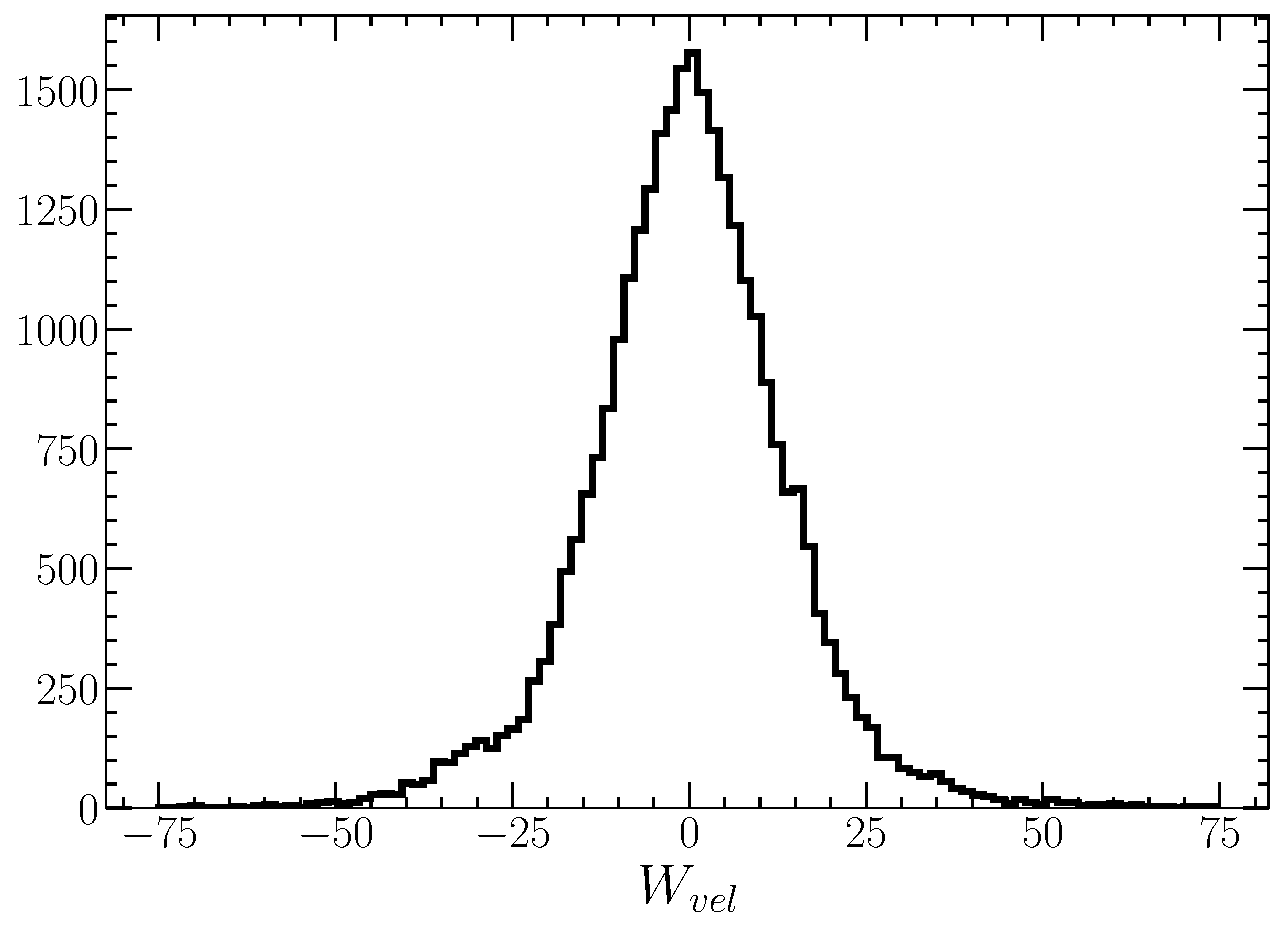
\includegraphics[width=0.75\textwidth]{src/Figures/WvelDist.pdf}
	\caption{Distribution of vertical velocity displacement from \citet{Lu2021}.}
	\label{fig:LuKde}
\end{figure}
